\documentclass[a4paper,11pt]{article}

\usepackage[utf8]{inputenc}
\usepackage[T1]{fontenc}
\usepackage[francais]{babel}
\usepackage{amsmath,amssymb}
\usepackage{xspace}
\usepackage{graphicx}
\usepackage{verbatim}
\usepackage{listings}
\usepackage[usenames,dvipsnames]{color}
\usepackage{hyperref}

\title{Projet Unix}
\author{Nathan GUYOT \and Vincent LEFOULON}

% ===============
\begin{document}
% ===============
\maketitle

\section{Le code}

Dans les grandes lignes, le code s'organise autour d'une boucle : celle parcourant
les images du dossier source. Cette boucle se base sur les indices et non directement
sur les éléments (stockés dans un \verb+array+) afin de pouvoir plus facilement
récupérer les images adjacentes.

A chaque tour de boucle, on crée la miniature, puis génère la page d'aperçu et enfin ajoute l'image au fichier HTML.

\section{Le Makefile}

Le graphe des tâches est le suivant :

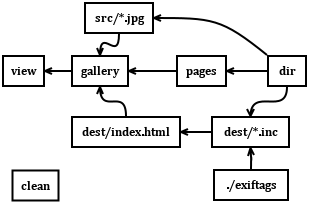
\includegraphics[width=320px]{MakefileGraph.png}

Chaque règle se contente d'appeler un script shell de la forme \verb+make-X.sh+, lequel analyse ses paramètres et exécute un des scripts implémentés dans la première version de la galerie.

\section{Mesure du temps d'exécution}

La commande \verb+make clean; time make gallery+ affiche :

\begin{verbatim}
real  0m0.761s
user  0m0.610s
sys 0m0.053s
\end{verbatim}

La parallélisation donne :

\begin{verbatim}
$ make clean; time make -j 14 gallery
real  0m0.538s
user  0m1.153s
sys 0m0.140s

$ make clean; time make -j 12 gallery
real  0m0.557s
user  0m1.230s
sys 0m0.147s

$ make clean; time make -j 10 gallery
real  0m0.544s
user  0m1.127s
sys 0m0.190s

$ make clean; time make -j 8 gallery
real  0m0.503s
user  0m1.087s
sys 0m0.147s

$ make clean; time make -j 6 gallery
real  0m0.529s
user  0m1.133s
sys 0m0.177s

$ make clean; time make -j 4 gallery
real  0m0.509s
user  0m1.143s
sys 0m0.160s

$ make clean; time make -j 2 gallery
real  0m0.529s
user  0m0.867s
sys 0m0.110s
\end{verbatim}

\section{Les données EXIF}

Les suffixes dans les Makefiles sont obsolètes, notamment parce qu'ils ne permettent pas ne
définir de dépendances. Dans le cas présent, les fichiers \verb+.c+ n'ont donc
pas pour dépendance le \verb+.h+ correspondant. On pourrait plutôt faire :

\begin{verbatim}
%.c: %.h

%.o: %.c
	$(CC) $(CFLAGS) -o $@ -c $<
\end{verbatim}

% =============
\end{document} 
% =============
